\section{Logika (back-end)}
\label{Chapter66}

System \textit{iQuest} do prawidłowej pracy wymagał zaprogramowania odpowiedniej logiki biznesowej, rozwiązującej stawiane przed nim zadania. Najważniejszym zagadnieniem w kategorii logiki systemu jest interakcja z bazą danych. Poza nią, system posiada: procesor zadań wykonywanych w tle, oparty na \textit{CRON}; moduły odpowiadające za komunikację z systemami uczelanianymi -- m.in. \textit{ePoczta} i \textit{eDziekanat}; moduł logowania zdarzeń. W trakcie implementacji, zdecydowano się nie tworzyć osobnego mechanizmu do przechowywania ustawień w bazie danych, wykorzystując do tego celu funkcjonalność dostępną już w \textit{Moodle}. \\

Jedno z wymagań pozafunkcjonalnych dotyczyło zastosowania bazy danych \textit{PostgreSQL}. Platforma \textit{Moodle} korzysta z mechanizmu \emph{XMLDB}, co pozwala na ominięcie wielu problemów pojawiających się przy migracjach pomiędzy różnymi systemami baz danych. Niestety kosztem wykorzystania tego mechanizmu jest konieczność pracy z interfejsami programowania aplikacji dostarczanym przez platformę \textit{Moodle} -- \textit{Data manipulation API}. Na diagramach \ref{rys:back-end1}. oraz \ref{rys:back-end2}. przedstawiających wyżej opisaną logikę systemu \textit{iQuest}, znajdują się także klasy przechowujące stałe: \textit{tables} oraz \textit{settings}. \\

\begin{figure}[H]
\begin{center}
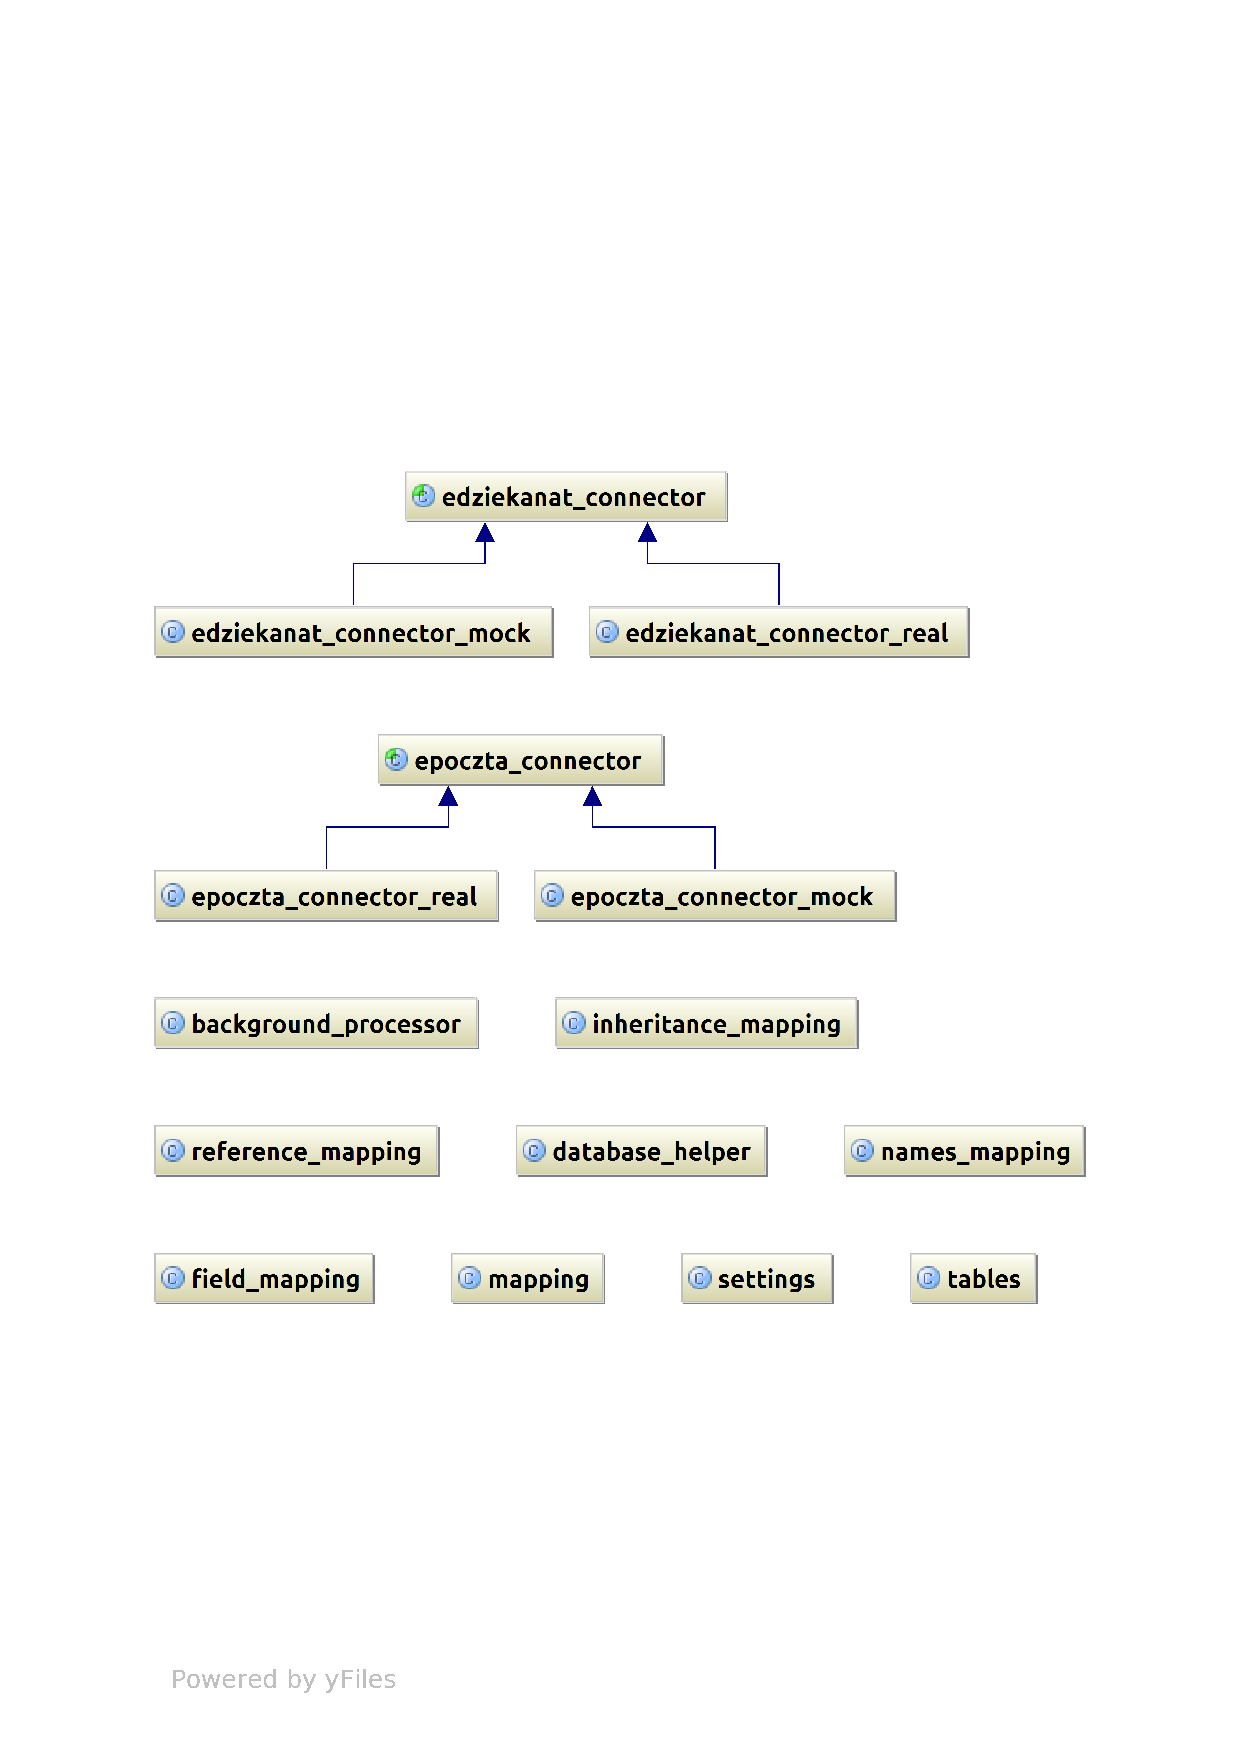
\includegraphics[width=0.9\textwidth]{figures/lw/backend1.pdf} 
\end{center}
\caption{Struktura back-end'u (1)}\label{rys:back-end1}
\end{figure}

\newpage
\begin{figure}[H]
\begin{center}
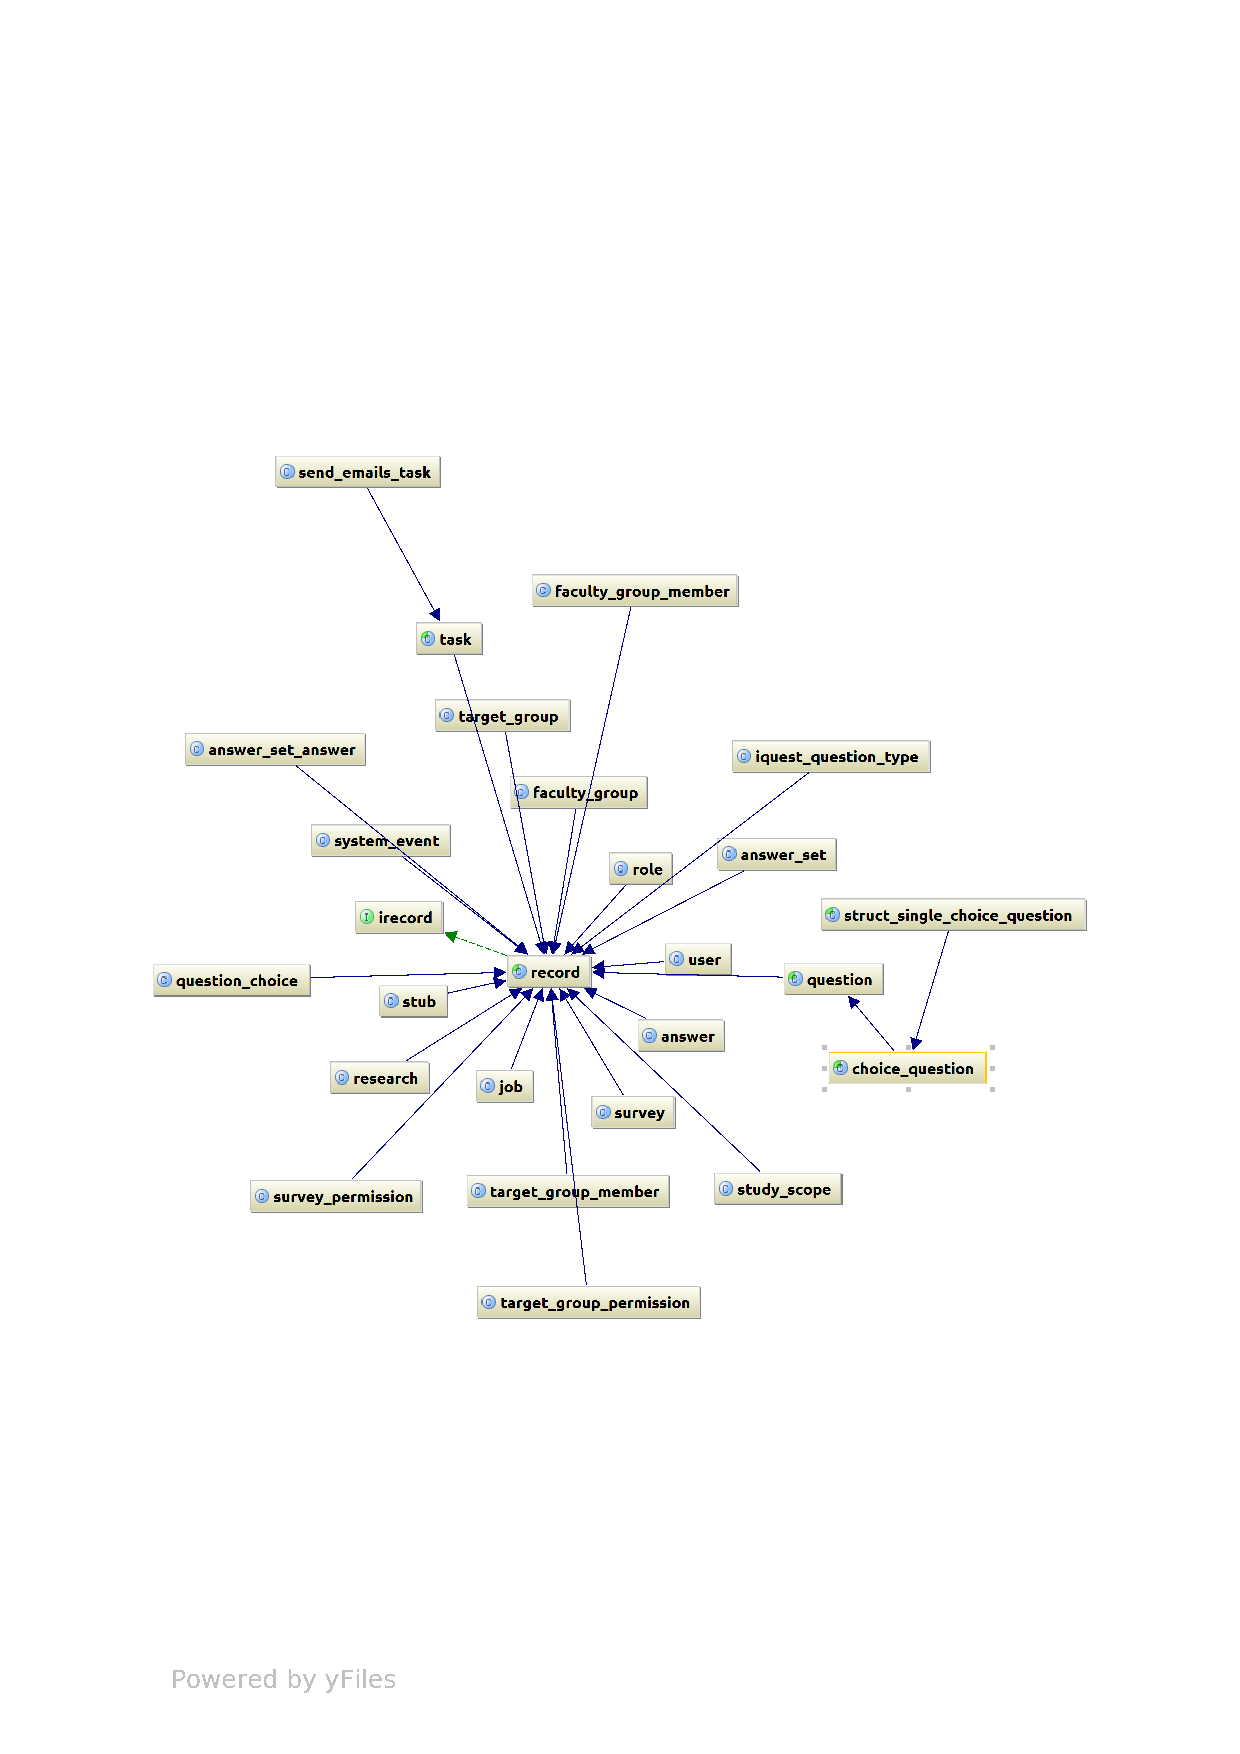
\includepdf{figures/lw/backend2.pdf} 
\end{center}
\caption{Struktura back-end'u (2)}\label{rys:back-end2}
\end{figure}
\newpage

\subsection{Raporty}
Raporty wykonano z użyciem platformy \textit{JasperReports}, wykorzystując następujące produkty firmy \textit{Jaspersoft}:

\begin{description}
\item[JasperReports Server] (wersja 5.0) -- serwer usług raportowania, na którym przechowywane są przygotowane przez zespół artefakty, służące umożliwieniu generacji raportów osobom dysponującym odpowiednimi uprawnieniami. Wykorzystano następujące funkcjonalności: definiowania źródła danych, raportu, ładowania plików z projektem raportu, zasobami oraz z generacji raportu.
\item[Jaspersoft Studio] (wersja 1.3.2) -- bazowane na Eclipse narzędzie, służące projektowaniu raportów. Z jego użyciem przygotowano projekty raportów w formacie \textit{JRXML}.
\end{description}

Kody źródłowe pakietu \textit{JasperReports} są pisane w języku \textit{Java}. Źródłem danych dla raportu, jest przygotowana przez zespół implementacja interfejsu \textit{ReportDataSourceService} z \textit{API JasperServer}. Źródło danych łączy się z usługami zdalnymi udostępnianymi przez wskazaną instancję systemu \textit{iQuest}, z których otrzymuje informacje o przeprowadzanych badaniach. Do tego celu, korzysta z protokołu SOAP. Struktura raportu zależy od typu pytania (otwarte\slash zamknięte). W przypadku pytań otwartych, prezentowana jest lista odpowiedzi. Dla pytań zamkniętych, na podstawie pobranych danych, generowane są statystyki, przekazywane następnie do podraportu w postaci obiektu klasy \textit{JRBeanCollectionDataSource}. W generacji statystyk z danych badań wykorzystano bibliotekę \textit{JoSQL}. \\

Definicja projektu raportu składa się z czterech plików, odpowiadających trzem poziomom:

\begin{description}
\item[researches.jrxml] -- raport główny dla badań.
\item[questions.jrxml] -- podraport dla pytań.
\item[answers\_closed.jrxml] -- podraport odpowiedzi zamkniętych.
\item[answers\_open.jrxml] -- podraport dla odpowiedzi otwartych.
\end{description}

Do generacji namiastek obiektów zdalnych (ang. \definicja{stub}) wykorzystano \textit{Apache Axis}. Wygenerowane klasy dostosowano tak, by akceptowały obiekty z zadanej instancji \textit{iQuest} oraz dla zmiennej przestrzeni nazw (ang. \definicja{namespace}). \\

W trakcie generacji \textit{stub'ów} okazało się, iż definicja usług dla protokołu \textit{SOAP} w języku \textit{WSDL} (ang. \definicja{Web Service Description Language}) generowana przez \textit{Moodle} jest niepoprawna. Skorzystano zatem z poprawionej wersji z zewnętrznego źródła: \url{https://github.com/ghigio/moodle-webservice_soapfda}. \\

Dostęp do usług zdalnych definiowanych w \textit{Moodle} zabezpieczono korzystając z mechanizmu generacji tokenu dla wybranego użytkownika. Użytkownik, który z poziomu serwera \textit{Jasper Server} zamierza wygenerować raport, musi znać adres systemu oraz posiadać token dostępu do usługi.

\subsection{Moduły uwierzytelniania}
Korzystając z mechanizmów rozszerzeń \textit{Moodle} zaimplementowano dwa moduły uwierzytelniania, tj.:

\begin{description}
\item[eKontoAuthenticationPlugin] -- integruje logowanie przez \textit{eKonto} z systemem \textit{iQuest},
\item[emailgraduate] -- pozwala absolwentom uczelni na rejestrację z użyciem adresu e-mail.
\end{description}

W celu spełnienia wymagań Działu Rozwoju Oprogramowania Politechniki Poznańskiej odnośnie wygaszania sesji użytkownika \textit{eKonto} po zadanym czasie (np.~15~minut), zmodyfikowano pliki źródłowe \textit{Moodle}, gdyż dla kodu odnoszącego się do sesji użytkownika \textit{Moodle} nie została przewidziana możliwość rejestracji rozszerzeń. Relacja \textit{user} została rozszerzona o opcjonalne pola związane z \textit{eKonto}, a jako że kod odpowiedzialny za manipulację schematem bazy danych nie jest wykonywany podczas instalacji modułu uwierzytelniania, umieszczono go w osobnym module (\textit{ekontodb}). \textit{eKontoAuthenticationPlugin} może być instalowany bez konieczności instalacji \textit{iSurvey}. Podczas jego implementacji korzystaliśmy z dokumentu \textit{Centralne uwierzytelnianie i wymiana danych. Wersja 1.2 (2010.07.06)}\cite{PP:CUiWD10}. \\

Podczas rejestracji z użyciem modułów systemu \textit{iQuest} użytkownik jest przydzielany do grupy docelowej ,,Absolwenci'', nadawana jest mu też rola respondenta w kontekście \textit{kursu iQuest}. Utworzenie modułu wiąże się z przygotowaniem klasy dziedziczącej z \textit{auth\_plugin\_base}, formularza ustawień, pliku lokalizacji oraz wersji.

\subsection{Moduły dla serwisów zewnętrznych}
\begin{description}
\item[ePocztaConnector] -- służy do wysyłania e-maili z serwera Politechniki Poznańskiej,
\item[eDziekanatConnector] -- pobiera i aktualizuje lokalne informacje o grupach dziekańskich, zakresach tematycznych tychże grup oraz ich studentach.
\end{description}

\textit{Dział Rozwoju Oprogramowania} udostępnia klienty \textit{eUsług} dla różnych języków, w tym dla \emph{PHP}. Komunikacja z usługami zdalnymi uczelni odbywa się poprzez protokół \textit{SOAP}. Wyżej wymienione moduły zaimplementowano z wykorzystaniem fabryki obiektów, która w zależności od trybu (testowy\slash produkcyjny) zwraca obiekt odpowiedniej klasy. Zadania związane z oba modułami są zlecane procesorowi zadań w tle.